\documentclass{article}
\usepackage[utf8]{inputenc}
\usepackage{subcaption}
\usepackage{wrapfig}
\usepackage{graphicx}
\usepackage{float}
\graphicspath{ {images/} }
\usepackage[margin=1in]{geometry}
\usepackage{url}
\usepackage{tikz}
\usetikzlibrary{arrows,automata,positioning}

\title{Sensores, dados e decisão}
\date{21 de Outubro de 2016}
\author{Bernardo Meurer\\
        \texttt{86242}
        \and
        Maria Adelaide Ambrósio\\
        \texttt{87064}
        \and
        Inês Coelho\\
        \texttt{87022}}
\begin{document}
\maketitle
\newpage

\subsection*{1. Backwards e Forwards}
\begin{wrapfigure}{R}{0.3\textwidth}
    \centering
    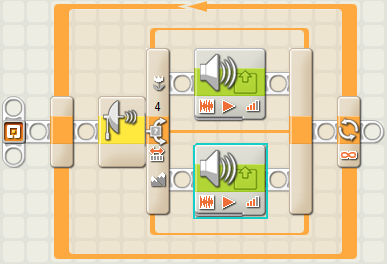
\includegraphics[width=0.3\textwidth]{bandf}
    \caption{Backwards and forwards}
\end{wrapfigure}
O robô deverá dizer `forward' quando está a uma distância superior a 40cm do
obstáculo e `backward' quando a distância for inferior a este valor. Para o
efeito utilizamos um programa que consiste num loop que envolve um bloco de
decisão associado ao sensor ultrasónico de distância. Configuramo-lo escrevendo
o parâmetro da distância padrão (40cm). Finalmente, acrescentamos os blocos
de altifalante com os sons a serem gerados em cada um dos casos (“Forward” e
“Backward”). Colocamos estes blocos nos dois ramos da saída do bloco de decisão.
\newline

\subsection*{2. MatLAb}
\begin{figure}[H]
    \centering
    \begin{subfigure}{.5\textwidth}
        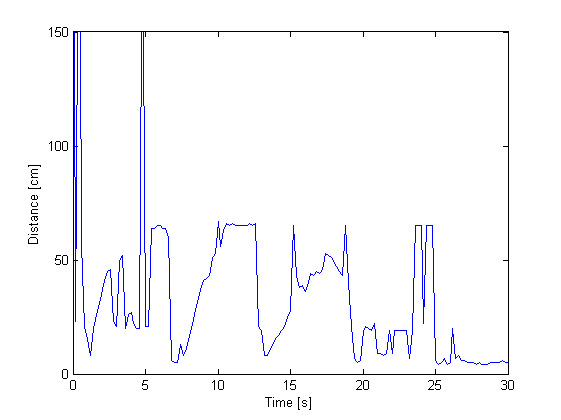
\includegraphics[scale=.5]{ultra}
        \caption{Distância em função do tempo}
    \end{subfigure}%
    \begin{subfigure}{.5\textwidth}
        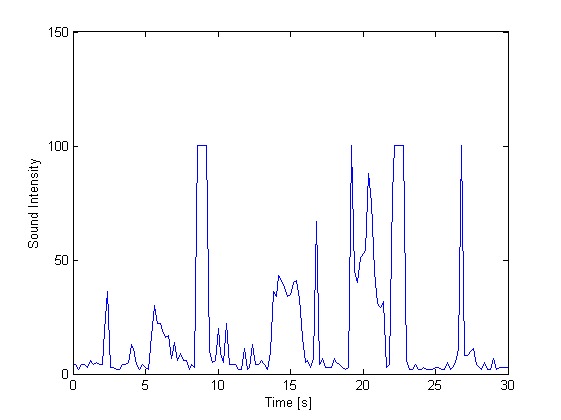
\includegraphics[scale=.5]{sound}
        \caption{Intensidade do som em função do tempo}
    \end{subfigure}%
    \newline

    \begin{subfigure}{.5\textwidth}
        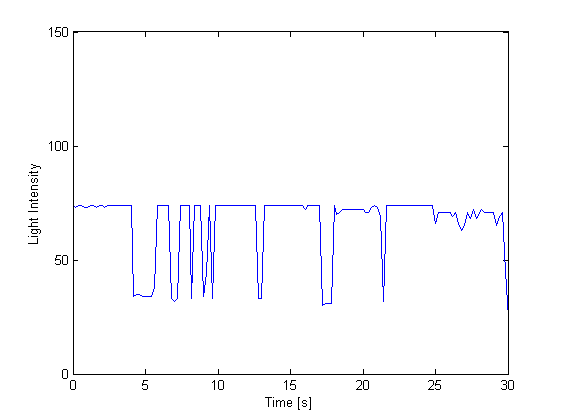
\includegraphics[scale=.5]{light}
        \caption{Intensidade da luz em função do tempo}
    \end{subfigure}
\end{figure}
\subsection*{2.1 Descrição dos ensaios}
Para cada um dos ensaios variámos as situações de estudo, isto é: no caso do estudo da
intensidade do som mudámos o tipo de som produzido (batemos palmas, estalamos os dedos,
fizemos sons agudos, etc); no caso da intensidade da luz utilizámos pequenos retângulos de
cartolina branca e preta para variar a taxa de reflexão da luz. Por último relativamente à
distância, afastamos e aproximamos um objeto sucessivamente. Em todos os casos observamos que os
gráficos refletiam as variações efetuadas
\subsection*{3. Valor da Constante}
O valor da constante responsável por corrigir os valores em polegadas para centímetros é a taxa
de conversão 1' = 2.54cm.
\subsection*{4. Paragem Suave}
O programa ``Paragem Suave'' é um caso particular de um programa que mantém o robot a uma certa
distância da parede pois é simplesmente uma modificação deste de forma a modular a intensidade
de funcionamento do motor, além de realizar a ação de parada.
\begin{figure}[H]
    \centering
    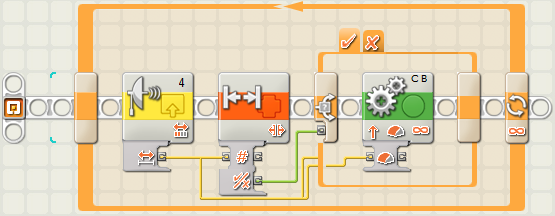
\includegraphics[scale=.5]{paragem-suaved}
    \caption{O código do programa Paragem Suave}
\end{figure}
\end{document}
